% Options for packages loaded elsewhere
\PassOptionsToPackage{unicode}{hyperref}
\PassOptionsToPackage{hyphens}{url}
%
\documentclass[
]{article}
\usepackage{amsmath,amssymb}
\usepackage{iftex}
\ifPDFTeX
  \usepackage[T1]{fontenc}
  \usepackage[utf8]{inputenc}
  \usepackage{textcomp} % provide euro and other symbols
\else % if luatex or xetex
  \usepackage{unicode-math} % this also loads fontspec
  \defaultfontfeatures{Scale=MatchLowercase}
  \defaultfontfeatures[\rmfamily]{Ligatures=TeX,Scale=1}
\fi
\usepackage{lmodern}
\ifPDFTeX\else
  % xetex/luatex font selection
\fi
% Use upquote if available, for straight quotes in verbatim environments
\IfFileExists{upquote.sty}{\usepackage{upquote}}{}
\IfFileExists{microtype.sty}{% use microtype if available
  \usepackage[]{microtype}
  \UseMicrotypeSet[protrusion]{basicmath} % disable protrusion for tt fonts
}{}
\makeatletter
\@ifundefined{KOMAClassName}{% if non-KOMA class
  \IfFileExists{parskip.sty}{%
    \usepackage{parskip}
  }{% else
    \setlength{\parindent}{0pt}
    \setlength{\parskip}{6pt plus 2pt minus 1pt}}
}{% if KOMA class
  \KOMAoptions{parskip=half}}
\makeatother
\usepackage{xcolor}
\usepackage[margin=1in]{geometry}
\usepackage{longtable,booktabs,array}
\usepackage{calc} % for calculating minipage widths
% Correct order of tables after \paragraph or \subparagraph
\usepackage{etoolbox}
\makeatletter
\patchcmd\longtable{\par}{\if@noskipsec\mbox{}\fi\par}{}{}
\makeatother
% Allow footnotes in longtable head/foot
\IfFileExists{footnotehyper.sty}{\usepackage{footnotehyper}}{\usepackage{footnote}}
\makesavenoteenv{longtable}
\usepackage{graphicx}
\makeatletter
\def\maxwidth{\ifdim\Gin@nat@width>\linewidth\linewidth\else\Gin@nat@width\fi}
\def\maxheight{\ifdim\Gin@nat@height>\textheight\textheight\else\Gin@nat@height\fi}
\makeatother
% Scale images if necessary, so that they will not overflow the page
% margins by default, and it is still possible to overwrite the defaults
% using explicit options in \includegraphics[width, height, ...]{}
\setkeys{Gin}{width=\maxwidth,height=\maxheight,keepaspectratio}
% Set default figure placement to htbp
\makeatletter
\def\fps@figure{htbp}
\makeatother
\setlength{\emergencystretch}{3em} % prevent overfull lines
\providecommand{\tightlist}{%
  \setlength{\itemsep}{0pt}\setlength{\parskip}{0pt}}
\setcounter{secnumdepth}{5}
\newlength{\cslhangindent}
\setlength{\cslhangindent}{1.5em}
\newlength{\csllabelwidth}
\setlength{\csllabelwidth}{3em}
\newlength{\cslentryspacingunit} % times entry-spacing
\setlength{\cslentryspacingunit}{\parskip}
\newenvironment{CSLReferences}[2] % #1 hanging-ident, #2 entry spacing
 {% don't indent paragraphs
  \setlength{\parindent}{0pt}
  % turn on hanging indent if param 1 is 1
  \ifodd #1
  \let\oldpar\par
  \def\par{\hangindent=\cslhangindent\oldpar}
  \fi
  % set entry spacing
  \setlength{\parskip}{#2\cslentryspacingunit}
 }%
 {}
\usepackage{calc}
\newcommand{\CSLBlock}[1]{#1\hfill\break}
\newcommand{\CSLLeftMargin}[1]{\parbox[t]{\csllabelwidth}{#1}}
\newcommand{\CSLRightInline}[1]{\parbox[t]{\linewidth - \csllabelwidth}{#1}\break}
\newcommand{\CSLIndent}[1]{\hspace{\cslhangindent}#1}
\usepackage{setspace}\doublespacing
\usepackage{booktabs}
\usepackage{longtable}
\usepackage{array}
\usepackage{multirow}
\usepackage{wrapfig}
\usepackage{float}
\usepackage{colortbl}
\usepackage{pdflscape}
\usepackage{tabu}
\usepackage{threeparttable}
\usepackage{threeparttablex}
\usepackage[normalem]{ulem}
\usepackage{makecell}
\usepackage{xcolor}
\ifLuaTeX
  \usepackage{selnolig}  % disable illegal ligatures
\fi
\IfFileExists{bookmark.sty}{\usepackage{bookmark}}{\usepackage{hyperref}}
\IfFileExists{xurl.sty}{\usepackage{xurl}}{} % add URL line breaks if available
\urlstyle{same}
\hypersetup{
  pdftitle={Avoiding global deforestation by taxing land in agricultural production: The implications for global markets},
  pdfauthor={Eric C. Davis, Maros Ivanic, and Brent Sohngen},
  hidelinks,
  pdfcreator={LaTeX via pandoc}}

\title{Avoiding global deforestation by taxing land in agricultural production: The implications for global markets}
\author{Eric C. Davis, Maros Ivanic, and Brent Sohngen}
\date{February 28, 2024}

\begin{document}
\maketitle
\begin{abstract}
The projected growth in population and incomes is expected to create pressure to convert forestland into farmland. At the same time, the increasingly negative climate impacts are expected to generate further pressure to enhance the terrestrial carbon sink. Even though these goals are incompatible as reversing the deforestation trend by afforesting cropland would result in negative market impacts such as higher food prices, using the GTAP and GTM models, we find that these impacts would be relatively small if the goal of preserving 144.2 million hectares of forestland that otherwise would be converted to agricultural land by 2033 is achieved through a tax on using land in agricultural production. As to the economic price for doing so, the avoided deforestation would in most regions of the world result in less agricultural output and higher market prices. This is estimated to impact the well-being of global consumers by \$92.1 billion, which translates to a global average cost of \$10.6 per person in 2033.
\end{abstract}

\vspace{1in}

\textbf{The findings and conclusions in this publication are those of the author(s) and should not be construed to represent any official USDA or U.S. Government determination or policy.}

\textbf{This research was supported in part by the U.S. Department of Agriculture, Economic Research Service.}

\newpage

\hypertarget{introduction}{%
\section{Introduction}\label{introduction}}

In 2020, there were 4.1 billion hectares of forestland globally covering roughly 31.4\% of the land (FAO and UNEP 2020). These forests play an important role in maintaining and growing the land-based carbon sink by sequestering about 30\% of GHG emissions currently (Roe et al. 2019). This is because of forests proven ability to sequester carbon not only in the stems of trees (Davis, Sohngen, and Lewis 2022) but in their soils as well (Guo et al. 2021). With increasingly negative climate impacts, the pressure to enhance the terrestrial sink is growing, and one of the tools to achieve this is afforestation. As such, there is growing attention being placed globally to afforestation efforts, which is highlighted by the UN's declaration of the years from 2021 through 2030 as the UN Decade of Ecosystem Restoration (Sewell, Esch, and Lowenhardt 2020). Many of the Nationally Determined Contributions (NDCs) countries have submitted, which detail their plans to keep warming under the 2C threshold, also rely to a significant degree on afforestation projects (Roe et al. 2019).

The global gains that can be realized from afforestation, however, are uncertain, with broad estimates of cumulative sequestration ranging from 42 gigatonnes to 700 gigatonnes by the end of the century (Bastin et al. 2019a, 2019b; Humpenöder et al. 2014; Sathaye et al. 2006; Doelman et al. 2020). In addition, the amount of land conversion that would be required also varies greatly, with estimates ranging from 0.3 billion hectares to 2.8 billion hectares (Bastin et al. 2019a, 2019b; Humpenöder et al. 2014; Doelman et al. 2020). In many cases, these results suggest massive losses in the amount of pasture and cropland that would be available. This puts into question the feasibility of attaining these results, as almost 90 percent of deforestation worldwide is undertaken to expand the amount of agricultural land (FAO 2021). There are many reasons for this. For example, as nations develop and disposable incomes rise, consumers often change to more meat-based diets. Population growth is also a driver. Currently, the United Nations' medium variant population projections suggest that between 2023 and 2033 the worlds' population will grow by 8.8 percent, a gain of 707.1 million people (Nations 2023). And where population growth is especially high, which is the case at present throughout most of Africa (2023 to 2033 population growth: 25.0\%: 360.6 million), this puts extreme pressure on policymakers to allow greater conversion of forestland into farmland. Still, some research has suggested that substantive gains in the carbon sink (+23.8PgCo2e/yr) can be made without sacrificing agricultural land (Griscoma et al. 2017).

If such efforts are to be made, it is important to understand where to target them, as afforestation is thought to not provide equal benefits in every region. For example, afforestation in boreal zones has been shown to provide the smallest net benefits, as the carbon sequestrations benefits of conifer forests are mitigated by the reduction in albedo in winter (Mykleby, Snyder, and Twine 2017; Li et al. 2015). Coniferous forests have also been shown to increase soil organic carbon less than broadleaf forests (Guo et al. 2021). Conversely, tropical forests have been linked with a strong positive result from afforestation, as the carbon sequestration benefit is complemented by a cooling impact due to changes in both albedo and evapotranspiration, and with temperate forests, the impact of afforestation is also shown to be positive, albeit less strongly so due to a winter warming effect (Li et al. 2015).

South America and Sub-Saharan Africa are thus two regions that show much potential for afforestation. It is estimated that these two regions hold at least 50\% of the potential for global gains while regions such as Northern Africa and the Middle East show little promise as forest growth rates are quite low (Doelman et al. 2020). Thus, it is promising that the African Forest Landscape Restoration Initiative (AFR100), which aims to afforest 100 million hectares by 2030, has roughly 70\% of its commitments coming from Sub-Saharan nations (AUDA-NEPAD 2023). While many of these nations may be well-suited in biophysical terms for afforestation, there is concern about how long-lasting any investment may be due to proximate zones of political instability. There are other nations that have a big potential for gains from afforestation, but they also face challenges. India, for example, has a great potential to increase its carbon sequestration through afforestation, but its massive population and food security worries limit its ability to consider such actions. The United Nations suggests that India's population will grow slightly less fast than the world average between 2023 and 2033 (+8.5\%), but due to its sizable base, that will equate to an increase in population of 120.5 million. Thus, its NDC does not entertain the idea of agricultural land being re-purposed and instead primarily considers targeting wastelands that may not be well suited for afforestation (Amjath-Babu et al. 2019). Moreover, as land-use decisions in one country also tend to have impacts that spillover into many others (Meyfroidt, Rudel, and Lambin 2010; Lambin and Meyfroidt 2011), analysis needs to be conducted at a global scale.

Several notable modeling attempts have been made in this direction. Steinbuks and Hertel (2012) developed their global partial equilibrium FABLE model (Forestry, Agriculture, Biofuels, Land Use, and Environment) to identify the optimal land use choices given the competing demands of meeting greenhouse gas targets and satisfying demand for food, bioenergy, forest products, and ecosystem services. While FABLE is a powerful tool for examining the optimal trajectory of various land uses under specific demand assumptions, it is focused on specific sectors of the economy and neglects general equilibrium and household welfare effects (Steinbuks and Hertel 2012; Hertel 2017). Other efforts have used the Global Trade Analysis Project (GTAP) computable general equilibrium model to address such questions, but its standard model does not well account for land-use changes. This prompted the creation of the Land Use and Land Cover Database within the GTAP framework, which incorporates forestry remote-sensing products (Baldos and Hertel 2012). The GTAP Agro-Ecological Zone (GTAP-AEZ) model further strengthened the GTAP model's ability to analyze land use changes, with the use of spatially explicit global land use data and through the incorporation of intra- and inter-regional land and land-based greenhouse emissions heterogeneity (Hertel et al. 2008). While the GTAP-AEZ model benefits from the inclusion of competition among different crops, grazing, and forest-based uses, it has limitations, primarily due to its infrequent updates. The \href{mailto:KLUM@GTAP}{\nolinkurl{KLUM@GTAP}} framework integrated the Kleines Land Use Model (KLUM) with an extended yet static version of GTAP called GTAP-EFL to evaluate the impact of climate change on cropland allocation. KLUM is a global agricultural land-use model that connects the economy to global crop allocation to maximize producer returns under specific risk assumptions, and GTAP-EFL separates energy factors from intermediate inputs and incorporates them into capital, while also considering CO2 emissions. \href{mailto:KLUM@GTAP}{\nolinkurl{KLUM@GTAP}} substitutes the land allocation mechanism within GTAP-EFL by utilizing regionally aggregated area changes in cropland determined by KLUM to update cropland shares in GTAP-EFL (Ronneberger and Tol 2009).

More recent modeling attempts of land-use change have begun to move away from comparative static analysis though. For example, the dynamic GTAP model, supported by the GTAP-AEZ database, considers land market effects, which were identified as significant in driving results by Stevenson (2013). This model has been utilized to evaluate the impact of crop intensification on land use. It, however, has been critiqued, as global aggregates may mask localized shifts that can have implications for ecologically significant areas (Byerlee 2014). In addition, in the standard GTAP model, it is difficult to model a sector individually. There are 68 market sectors covered in the latest version of the GTAP database. The GTAP model's general equilibrium nature means that all these markets are cleared with market-clearing prices. As the model applies nested CES production functions to all sectors and differentiates them by parameters only, to model one sector, in this case forestry, differently from the rest would require a major redesign of the model. While not impossible, this project will attempt to get around these concerns and assess the impact of various likely land-use scenarios by melding the dynamic GTAP model with the Global Timber Model (GTM), which is a dynamic optimization model that has been specifically designed to analyze the relationship among land rents, forested land cover, and carbon sequestration through forests and thus is better able to examine the impact of afforestation or avoided deforestation on the carbon sink (Sohngen, Mendelsohn, and Sedjo 2001). The latest versions of both models were used. For the GTAP model, this meant using data which has 2017 as its base year. This data was then updated to the base year (2023) using data from the Centre for Prospective Studies and International Information (CEPII) (Fontagné and Santoni 2022) to account for the projected changes in gross domestic product (GDP), population, and productivity for each country in the world. Similar steps were taken to update and recalibrate the GTM model.

\hypertarget{connecting-the-gtap-and-gtm-models}{%
\section{Connecting the GTAP and GTM models}\label{connecting-the-gtap-and-gtm-models}}

Both the GTAP and GTM models represent widely used models for policy analysis. In the case of GTAP, the model is used to describe the implications of various policy instruments for national and globla markets, including prices, output and trade. The GTM model is, on the other hand, capable to translating the impacts of population and global growth, and the changes in land returns, to changes in global forested areas and calculate the impacts on total carbon contained in forests.

Even though the GTAP and GTM models capture important aspects of the global economy and the biophysical world, they do not contain certain behaviors. In the case of GTAP, the model assumes that the amount of agricultural land is fixed, while the GTM considers the returns to land fixed. By combining the two models, we can fill each model missing behavior for a more complete description of the global impacts.

The combination of the two models means that we use the GTAP model to create the link between the amounts of available land and its returns for the benefit of the GTM model, while at the same time we use the GTM model to create the response of agricultural land quantity to returns in land returns for the benefit of the GTAP model. By solving both models together, we can greatly expand the descriptive power of both models.

We achieve the combined solution of GTAP and GTM by passing outputs back and forth between the models until a dual-state equilibrium is achieved. Establishing a connection between the GTAP model and the GTM model requires that we model the return on land using the GTAP model and feed those results into the GTM model as exogenous inputs. The GTM model then endogenously determines the amount of land available for crop and livestock production, and we feed that back into the GTAP model as an exogenous input.

On the software level, we establish the connection between the models using an R script, which is capable of handling other software, including generating required inputs, executing it and reading in any outputs. This is required to operate the GTAP model, which is written in GEMPACK, and the GTM model, which is written in GAMS. As GEMPACK and GAMS were developed long before software integration became important or even possible, we use much more modern technologies made available through the R software (R Core Team 2021) to create the user functions that execut both models, collect their outputs, and automatically create any required input files.

\hypertarget{changes-under-the-baseline-projections}{%
\section{Changes under the baseline projections}\label{changes-under-the-baseline-projections}}

To understand the impact of potential regional and global afforestation actions, an important first step was creating a realistic baseline scenario that depicts the likely changes over the decade under study, 2023--2033. Data for this were drawn from CEPII (Fontagné and Santoni 2022). To build our scenario, we use two of their variables that we determined to be key: population and GDP. The CEPII projections do not contain any information on land use. To build a more complete baseline, we also include the projections on forested land change included in the Global Timber Model (GTM). Using the GTAP model in connection with the GTM model (to assure that the changes in land are consistent between the two models), we calculate the overall change in factor quantity/productivity growth required to achieve the targeted values in 2033. In Table \ref{tab:baseline-growth}, we show the projected population and GDP growth per region. GDP increases for all regions of the world with the largest percentage changes occurring in South Asia (+308.6\%), China (+189.8\%), and Sub-Saharan Africa (+172.9\%). Population also is projected to grow in most regions with the largest changes happening in Sub-Saharan Africa (+55.7\%). Japan, Russia, and East Asia are projected to see their populations decline by 10.4\%, 4.7\%, and 2.6\%, respectively. As for the projected change in agricultural land, our baseline prjoections show significant growth in Oceania (+27.6\%), Rest of Latin America (+25.8\%), Sub-Saharan Africa (+17.4\%), Central America (+13.9\%), and Brazil (+13.9\%). Japan is the only nation that sees a significant decline (-34.9\%) in agricultural land, which is likely tied in part to the population decline just described.

\begin{table}
\centering
\caption{\label{tab:baseline-growth}GDP, population, and agricultural land growth under the baseline scenario (Source: CEPII and GTM)}
\centering
\begin{tabular}[t]{|>{}l|r|r|>{}r|}
\hline
  & Real GDP (\%) & Population (\%) & Agricultural land (\%)\\
\hline
Oceania & 52.7 & 24.0 & 27.6\\
\hline
China & 189.8 & 0.8 & 0.0\\
\hline
Japan & 20.6 & -10.4 & -34.9\\
\hline
East Asia & 46.0 & -2.6 & -1.1\\
\hline
SE Asia & 138.5 & 15.0 & 11.7\\
\hline
South Asia & 308.6 & 17.8 & 12.8\\
\hline
Canada & 41.3 & 15.2 & 2.6\\
\hline
United States & 38.6 & 10.6 & -0.5\\
\hline
Central America & 74.1 & 18.3 & 16.7\\
\hline
Brazil & 20.8 & 7.8 & 13.9\\
\hline
Other Latin America & 64.8 & 15.8 & 25.8\\
\hline
West/Central Europe & 25.4 & 0.9 & 4.5\\
\hline
EU II & 113.1 & 8.7 & 3.1\\
\hline
Russia & 41.8 & -4.7 & 4.4\\
\hline
Sub-Saharan Africa & 172.9 & 55.7 & 17.4\\
\hline
North Africa/Middle East & 58.2 & 27.8 & 7.8\\
\hline
ROW & 44.4 & 36.8 & 0.0\\
\hline
\end{tabular}
\end{table}

Focusing on the absolute area of the forested areas, as generated by the GTM model, we estimate that between 2023 and 2033, 144.2 million hectares (3.6\%) of global forests will be converted to agricultural lands with the largest decline expected to happen in Sub-Saharan Africa, which is estimated to lose 39.7 million hectares (7.0\%) of its forestland (Table \ref{tab:baseline-forest-change}). Southeast Asia, Brazil, and the rest of South America also see forestland shrink significantly, with decreases of 22.6 million hectares (9.3\%), 19.0 million hectares (3.8\%), and 23.5 million hectares (6.7\%), respectively. Conversely, the United States is estimated to add 1.3 million hectares (0.5\%) to its forestland.

\begin{table}
\centering
\begin{threeparttable}
\caption{\label{tab:baseline-forest-change}Forestland by region in 2023 and estimated change by 2033}
\centering
\begin{tabular}[t]{|>{}l|r|r|r|>{}r|}
\hline
  & Forestland in 2023 & Forestland in 2033 & $\Delta$ (Mha) & $\Delta$ (\%)\\
\hline
United States & 248.4 & 249.7 & 1.3 & 0.5\\
\hline
China & 164.6 & 164.8 & 0.1 & 0.1\\
\hline
Brazil & 498.2 & 479.2 & -19.0 & -3.8\\
\hline
Canada & 412.8 & 407.9 & -5.0 & -1.2\\
\hline
Russia & 838.1 & 828.6 & -9.5 & -1.1\\
\hline
West/Central Europe & 186.7 & 175.5 & -11.1 & -6.0\\
\hline
EU II & 40.1 & 36.1 & -4.1 & -10.1\\
\hline
South Asia & 47.8 & 42.5 & -5.3 & -11.0\\
\hline
Central America & 94.6 & 91.2 & -3.4 & -3.6\\
\hline
Other Latin America & 348.5 & 325.0 & -23.5 & -6.7\\
\hline
Sub-Saharan Africa & 564.6 & 525.0 & -39.7 & -7.0\\
\hline
SE Asia & 243.9 & 221.3 & -22.6 & -9.3\\
\hline
Oceania & 199.2 & 196.1 & -3.1 & -1.5\\
\hline
Japan & 23.7 & 26.9 & 3.2 & 13.7\\
\hline
North Africa/Middle East & 33.8 & 30.9 & -2.9 & -8.5\\
\hline
East Asia & 14.5 & 14.6 & 0.1 & 0.7\\
\hline
Total & 3959.5 & 3815.3 & -144.2 & -3.6\\
\hline
\end{tabular}
\begin{tablenotes}
\small
\item [a] Southeast Asia includes Brunei Darussalam, Cambodia, Indonesia, Laos, Malaysia, Myanmar, Philippines, Singapore, Thailand, Timor-Leste, and Vietnam.
\item [b] Oceania includes Australia, Cook Islands, Fiji, French Polynesia, Kiribati, Marshall Islands, Micronesia, Nauru, New Caledonia, New Zealand, Palau, Papua New Guinea, Samoa (Western Samoa), Solomon Islands, Tonga, Tuvalu, and Vanuatu.
\item [c] Rest of South America includes Argentina, Bolivia, Czech Republic, Chile, Colombia, Ecuador, the Falkland Islands, French Guiana, Guyana, Paraguay, Peru, South Georgia, the South Sandwich Islands, Suriname, Uruguay, and Venezuela.
\item [d] Western \& Central Europe includes  Austria, Belgium, Bulgaria, Croatia, Denmark, Estonia, Finland, France, Hungary, Iceland, Italy, Ireland, Germany, Greece, Latvia, Liechtenstein, Lithuania, Luxembourg, Malta, Monaco, Montenegro, Netherlands, North Macedonia, Norway, Poland, Portugal, Romania, Serbia, Slovakia, Slovenia, Spain, Sweden, Switzerland, Turkey, and the United Kingdom.
\item [e] Other Europe includes Albania, Armenia, Azerbaijan, Belarus, Bosnia and Herzegovina, Georgia,  Kosovo Kazakhstan, Kyrgyzstan, Moldova, Tajikistan, and Ukraine.
\end{tablenotes}
\end{threeparttable}
\end{table}

\hypertarget{modeling-the-impact-of-possible-measures-to-mitigate-deforestationpromote-afforestation}{%
\section{Modeling the impact of possible measures to mitigate deforestation/promote afforestation}\label{modeling-the-impact-of-possible-measures-to-mitigate-deforestationpromote-afforestation}}

Against the backdrop of the baseline scenario, we turn to the question of what policy could prevent global deforestation in the period of 2023--2033. Because the area of forestland is mostly determined by the relative returns of land in agriculture and forestry, in our policy scenario we modify the return to land in agriculture by applying a uniform global tax on the use of land in the production of agricultural output. Solving the two models together shows that it would require a tax of roughly 70 percent to be assessed on the use of land for the deforestation rate to fall globally to zero. The economic impact of such a policy measure would not be limited to the cost of the tax, it would also impact food production and its prices. For example, with this policy in place, most regions of the world would see significant declines in the amount of agricultural land in 2033 relative to the baseline scenario where land conversion was not taxed. For the United States, there would be 2.1 percent less agricultural land (Table \ref{tab:baseline-scenario1}). Larger decreases would happen in other major agricultural production regions such as China (-2.5 percent), South Asia (-7.9 percent), Brazil (-8.6 percent), and Russia (-9.3 percent).

These reductions in the amount of agricultural land would then impact the quantity of agricultural goods that could be produced. For example, the 15.0 percent decrease in agricultural land in East Asia and the 9.0 percent decrease in agricultural land in Southeast Asia would result in large declines in percentage terms in agricultural production of 5.0 percent and 1.7 percent, respectively. Surprisingly, Brazil and the United States, despite their decreases in available agricultural land compared to the baseline 2033 scenario, are estimated to see increased agricultural output of 0.6 percent and 1.0 percent, respectively. This may be tied to the sharp declines in other regions prompting greater intensity of production to satisfy external demand.

\begin{table}
\centering
\caption{\label{tab:baseline-scenario1}Changes in key variables relative to baseline under a uniform land tax of 70 \%}
\centering
\begin{tabular}[t]{|>{}l|r|r|r|>{}r|}
\hline
  & Real GDP (\%) & Agr. land (\%) & Agr. prices (\%) & Agr. output (\%)\\
\hline
Oceania & -0.1 & -23.9 & 2.8 & -2.5\\
\hline
China & 0.0 & -2.5 & 1.1 & 0.0\\
\hline
Japan & -0.3 & -60.8 & 7.8 & -6.3\\
\hline
East Asia & -0.2 & -15.0 & 5.4 & -5.0\\
\hline
SE Asia & -0.3 & -9.0 & 2.9 & -1.7\\
\hline
South Asia & -0.3 & -7.9 & 3.0 & -1.0\\
\hline
Canada & 0.0 & -7.9 & 0.7 & 1.9\\
\hline
United States & 0.0 & -2.1 & 0.7 & 1.0\\
\hline
Central America & -0.2 & -15.6 & 2.7 & -2.0\\
\hline
Brazil & -0.1 & -8.6 & 1.3 & 0.6\\
\hline
Other Latin America & -0.4 & -23.1 & 3.8 & -3.2\\
\hline
West/Central Europe & 0.0 & -6.1 & 1.0 & 0.7\\
\hline
EU II & -0.1 & -3.2 & 1.3 & 0.3\\
\hline
Russia & -0.1 & -9.3 & 1.1 & 0.3\\
\hline
Sub-Saharan Africa & -0.2 & -4.0 & 1.4 & -0.2\\
\hline
North Africa/Middle East & -0.1 & -10.2 & 2.0 & -0.7\\
\hline
ROW & 0.0 & 0.0 & 0.8 & 0.9\\
\hline
\end{tabular}
\end{table}

\begin{table}
\centering
\caption{\label{tab:unnamed-chunk-4}Percentage change in the amount of forested land in 2033 with deforestation mitigation policy in place (Source: Authors' calculations)}
\centering
\begin{tabular}[t]{|>{}l|r|r|r|>{}r|}
\hline
  & Forestland in 2023 & Forestland in 2033 & $\Delta$ (Mha) & $\Delta$ (\%)\\
\hline
United States & 248.4 & 254.8 & 6.4 & 2.6\\
\hline
China & 164.6 & 174.8 & 10.2 & 6.2\\
\hline
Brazil & 498.2 & 492.2 & -6.0 & -1.2\\
\hline
Canada & 412.8 & 423.2 & 10.4 & 2.5\\
\hline
Russia & 838.1 & 849.7 & 11.6 & 1.4\\
\hline
West/Central Europe & 186.7 & 191.1 & 4.5 & 2.4\\
\hline
EU II & 40.1 & 40.3 & 0.2 & 0.4\\
\hline
South Asia & 47.8 & 46.2 & -1.6 & -3.3\\
\hline
Central America & 94.6 & 94.9 & 0.3 & 0.3\\
\hline
Other Latin America & 348.5 & 348.1 & -0.3 & -0.1\\
\hline
Sub-Saharan Africa & 564.6 & 535.6 & -29.0 & -5.1\\
\hline
SE Asia & 243.9 & 240.5 & -3.5 & -1.4\\
\hline
Oceania & 199.2 & 199.0 & -0.1 & -0.1\\
\hline
Japan & 23.7 & 23.5 & -0.1 & -0.6\\
\hline
North Africa/Middle East & 33.8 & 34.9 & 1.1 & 3.4\\
\hline
East Asia & 14.5 & 15.8 & 1.3 & 9.3\\
\hline
Total & 3959.5 & 3964.9 & 5.3 & 0.1\\
\hline
\end{tabular}
\end{table}

When we examine how this impacts exports of agricultural goods, we find that exports from Japan and the United States grow the most, increasing 8.8 percent and 3.5 percent, respectively (Table 4). The regions where agricultural exports drop most significantly are East Asia, South Asia, Southeast Asia, and Central America who see decreases of 14.5 percent, 5.9 percent, 5.1 percent, and 5.0 percent, respectively.

\begin{figure}
\centering
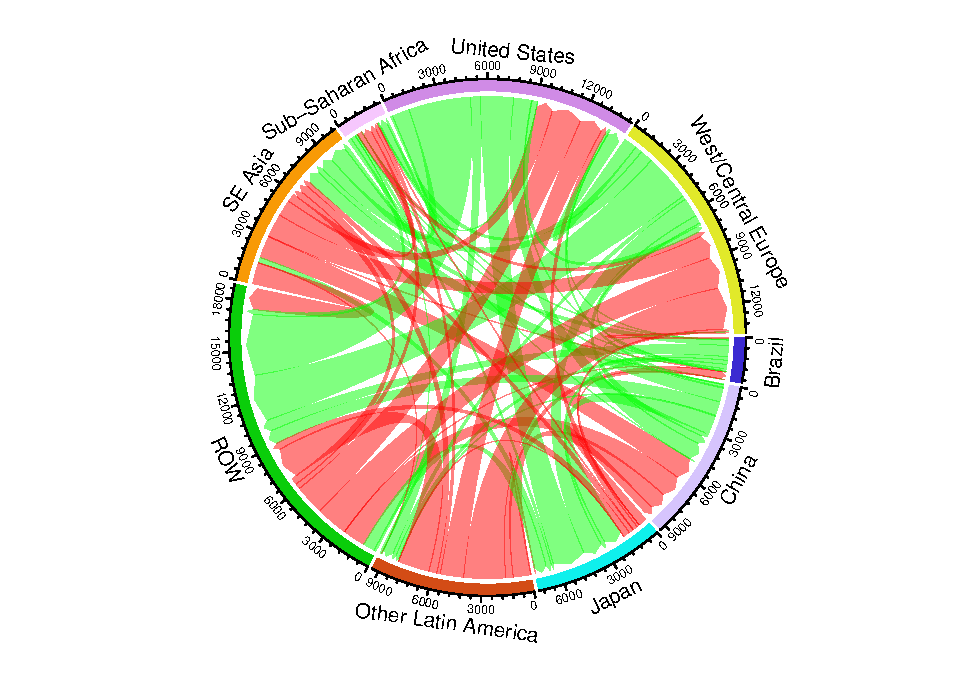
\includegraphics{paper_files/figure-latex/unnamed-chunk-5-1.pdf}
\caption{\label{fig:unnamed-chunk-5}Changes in ag trade volumes (red arrows denote reductions, green arrows denote increases)}
\end{figure}

Overall, this tax policy, which results in zero net deforestation globally, has a rather significant negative economic impact on all regions except Japan and Canada who see an increase in consumer well-being of \$977.1 million and \$166.9 million, respectively (Table \ref{tab:EV}). Consumer well-being is a measurement of equivalent variation and here measures the benefit/harm consumers experience in terms of income as a result of the policy changes. The United States, along with 10 other regions, see well-being drop by more than \$1 billion. The most negatively impacted regions are South Asia (-\$28.0 billion), China (-\$14.5 billion), and Southeast Asia (-\$13.6 billion). In total, this tax-driven policy is estimated to decrease global consumer well-being in 2033 by \$92.1 billion relative to the scenario where no tax on forestland conversion was in place.

\begin{table}
\centering
\caption{\label{tab:EV}Change in consumer well-being in 2033, by region, in billions dollars, with deforestation mitigation policy in place}
\centering
\begin{tabular}[t]{|>{}l|r|r|>{}r|}
\hline
  & Baseline (B\$) & Scenario (B\$) & $\Delta$ (B\$)\\
\hline
Oceania & 863.7 & 861.8 & -1.9\\
\hline
China & 23,275.9 & 23,260.0 & -15.9\\
\hline
Japan & 1,052.6 & 1,036.1 & -16.5\\
\hline
East Asia & 1,168.4 & 1,163.0 & -5.4\\
\hline
SE Asia & 3,886.2 & 3,872.4 & -13.9\\
\hline
South Asia & 9,493.4 & 9,465.6 & -27.8\\
\hline
Canada & 713.1 & 713.5 & 0.4\\
\hline
United States & 7,497.2 & 7,496.4 & -0.9\\
\hline
Central America & 1,241.2 & 1,236.4 & -4.8\\
\hline
Brazil & 423.0 & 422.4 & -0.6\\
\hline
Other Latin America & 1,242.6 & 1,233.2 & -9.4\\
\hline
West/Central Europe & 5,126.7 & 5,118.8 & -8.0\\
\hline
EU II & 839.3 & 838.7 & -0.6\\
\hline
Russia & 706.2 & 704.9 & -1.3\\
\hline
Sub-Saharan Africa & 2,766.7 & 2,758.8 & -7.8\\
\hline
North Africa/Middle East & 1,715.9 & 1,710.7 & -5.3\\
\hline
ROW & 13.9 & 13.9 & 0.0\\
\hline
Total & 62,026.3 & 61,906.6 & -119.7\\
\hline
\end{tabular}
\end{table}

Much of this loss in well-being may be the result of higher prices. Japan is the only nation that sees any price impacts that are beneficial for consumers resulting from this policy, with the price of agricultural goods decreasing 0.3 percent (Table \ref{tab:pm}). All other regions, for both agricultural and non-agricultural products, see prices rise between 0.3 and 5.1 percent.

\begin{table}
\centering
\caption{\label{tab:pm}Percent change in market prices for agricultural goods in 2033, with deforestation mitigation policy in place, relative to baseline}
\centering
\begin{tabular}[t]{|>{}l|>{}r|}
\hline
  & Ag prices\\
\hline
Oceania & 2.8\\
\hline
China & 1.1\\
\hline
Japan & 7.8\\
\hline
East Asia & 5.4\\
\hline
SE Asia & 2.9\\
\hline
South Asia & 3.0\\
\hline
Canada & 0.7\\
\hline
United States & 0.7\\
\hline
Central America & 2.7\\
\hline
Brazil & 1.3\\
\hline
Other Latin America & 3.8\\
\hline
West/Central Europe & 1.0\\
\hline
EU II & 1.3\\
\hline
Russia & 1.1\\
\hline
Sub-Saharan Africa & 1.4\\
\hline
North Africa/Middle East & 2.0\\
\hline
ROW & 0.8\\
\hline
\end{tabular}
\end{table}

\hypertarget{discussion}{%
\section{Discussion}\label{discussion}}

This analysis shows that, at an estimated tax rate of 70.3 percent of the value of each hectare of land that is converted to agricultural land, global net deforestation would drop to roughly zero by 2033, preserving 144.2 million hectares of forestland that otherwise would have been converted to agricultural land. In the United States, as USDA-NASS (Land Values 2022 Summary (August 2022)) valued the average hectare of farmland in 2022 at \$1,537.8, the tax would equate to \$1,081.1/hectare. In Brazil, CEIC valued the average price of Brazilian land at roughly 2,500 Brazilian Reals, which would put the tax at roughly \$82.2 per hectare. The economic price of this would likely be transfered to consumers through less agricultural output and higher market prices. Overall, such an action is estimated to reduce consumer well-being by \$92.1 billion or \$10.6 per every person in 2033. Governments might be wary of farmer discontent were they to take such fiscal actions and thus might be reluctant to impose such taxes on them. Thus, policymakers who wish to see deforestation stopped might have to resort to import tariffs on products produced on land converted from forestland for agricultural use.

We also show the utility of joining two major economic models. GTAP has long been valued for its ability to provide robust information on global trade flows and prices, and GTM has proven its utility in understanding the impact of forestry decisions on the carbon sink and land rents. By combining these models through the use of R and allowing the models to pass inputs and outputs back and forth iteratively, the benefits of both models have been maintained and their weaknesses greatly minimized. This advance holds great promise for advancement on a variety of fronts for researchers and policymakers interested in climate change, agricultural trade, and their inter-dependencies.

\hypertarget{conclusions}{%
\section{Conclusions}\label{conclusions}}

According to CEPII's projections, the growth of the global economy in the next ten years is expected to result in tremendous increases in global and regional GDP accompanied with a moderate growth in population. Another set of projections by GTM, however, suggests that this growth would also mean significant reductions in the world's forests that would be converted to agricultural land, resulting in a loss of over 100 million hectares of forest before 2033.

By combining two well known global models---the GTAP model that describes the world markets and trade, and the GTAM model that describes the impact of economic and population growth along with land rents on the amounts of forested areas---we were able to estimate the size of the tax on agricultural land needed to prevent deforestation in the coming ten years through reducing the returns to land when used in agriculture. We find that even though the tax is substantial at about 70 percent, it results in only very small reductions in the projected growth in global GDP and welfare. We also observe that the reduction in available agricultural land relative to the baseline growth results in reduced agricultural output and higher prices, which may require additional policy action to avoid negative impacts in terms of food security.

Finally, we note that a uniform global tax reducing the returns to land to the point of preventing global deforestation would produce highly differentiated impacts around the world's regions. Some regions, such as China, Russia, Canada and the United States would increase their forested areas as a result of the tax, while the regions with the greatest deforestation pressures, such as Sub-Saharan Africa, Brazil and Southeast Asia would only reduce the rate of their deforestation, for a zero change in the global forest area.

\newpage

\hypertarget{references}{%
\section{References}\label{references}}

\hypertarget{refs}{}
\begin{CSLReferences}{1}{0}
\leavevmode\vadjust pre{\hypertarget{ref-amjath2019}{}}%
Amjath-Babu, T. S., Pramod K. Aggarwal, Sonja Vermeulen Hans van Meijl, and Paul L. Lucas. 2019. {``Climate Action for Food Security in South Asia? Analyzing the Role of Agriculture in Nationally Determined Contributions to the Paris Agreement.''} \emph{Climate Policy} 19 (3). https://doi.org/\url{https://doi.org/10.1080/14693062.2018.1501329}.

\leavevmode\vadjust pre{\hypertarget{ref-auda2023}{}}%
AUDA-NEPAD. 2023. {``AFR100.''} \url{https://afr100.org}.

\leavevmode\vadjust pre{\hypertarget{ref-baldos2012}{}}%
Baldos, U. L. C., and Thomas W. Hertel. 2012. {``Development of a GTAP 8 Land Use and Land Cover Database for Years 2004 and 2007.''} \emph{GTAP Research Memorandum No. 23. Global Trade Analysis Project}.

\leavevmode\vadjust pre{\hypertarget{ref-veldman2019}{}}%
Bastin, Jean-Francois, Yelena Finegold, Claude Garcia, Danilo Mollicone, Marcelo Rezende, Devin Routh, Constantin M. Zohner, and Thomas W. Crowther. 2019a. {``Comment on "the Global Tree Restoration Potential".''} \emph{Science} 366 (6463).

\leavevmode\vadjust pre{\hypertarget{ref-bastin2019}{}}%
---------. 2019b. {``The Global Tree Restoration Potential.''} \emph{Science} 365 (6448).

\leavevmode\vadjust pre{\hypertarget{ref-byerlee2014}{}}%
Byerlee, Stevenson, D. 2014. {``Does Intensification Slow Crop Land Expansion or Encourage Deforestation?''} \emph{Global Food Security} 3 (2).

\leavevmode\vadjust pre{\hypertarget{ref-davis2022}{}}%
Davis, Eric C., Brent Sohngen, and David J. Lewis. 2022. {``The Effect of Carbon Fertilization on Naturally Regenerated and Planted US Forests.''} \emph{Nature Communications} 13 (1). https://doi.org/\url{https://doi.org/10.1038/s41467-022-33196-x}.

\leavevmode\vadjust pre{\hypertarget{ref-doelman2020}{}}%
Doelman, Jonathan C., Elke Stehfest, Detlef P. van Vuuren, Andrzej Tabeau, Andries F. Hof Maarten, C. Braakhekke, David E. H. J. Gernaat, et al. 2020. {``Afforestation for Climate Change Mitigation: Potentials, Risks and Trade‐offs.''} \emph{Global Change Biology} 26 (3).

\leavevmode\vadjust pre{\hypertarget{ref-fao2021}{}}%
FAO. 2021. {``COP26: Agricultural Expansion Drives Almost 90 Percent of Global Deforestation.''} \url{https://www.fao.org/newsroom/detail/cop26-agricultural-expansion-drives-almost-90-percent-of-global-deforestation/en}.

\leavevmode\vadjust pre{\hypertarget{ref-fao2023}{}}%
FAO, and UNEP. 2020. {``The State of the World's Forests 2020. Forests, Biodiversity and People.''} https://doi.org/\url{https://doi.org/10.4060/ca8642en}.

\leavevmode\vadjust pre{\hypertarget{ref-CEPII2024}{}}%
Fontagné, Perego, L., and G. Santoni. 2022. {``MaGE 3.1: Long-Term Macroeconomic Projections of the World Economy.''} \emph{International Economics} 172.

\leavevmode\vadjust pre{\hypertarget{ref-griscom2017}{}}%
Griscoma, Bronson W., Justin Adamsa, Peter W. Ellis, Richard A. Houghton, Guy Lomax, Daniela A. Miteva, William H. Schlesinger, et al. 2017. {``Natural Climate Solutions.''} \emph{Proceedings of the National Academy of Sciences} 114 (44).

\leavevmode\vadjust pre{\hypertarget{ref-guo2021}{}}%
Guo, Yang, Mohamed Abdalla, Mikk Espenberg, Astley Hastings, Paul Hallett, and Pete Smith. 2021. {``A Systematic Analysis and Review of the Impacts of Afforestation on Soil Quality Indicators as Modified by Climate Zone, Forest Type and Age.''} \emph{Science of the Total Environment} 757.

\leavevmode\vadjust pre{\hypertarget{ref-hertel2017}{}}%
Hertel, Thomas W. 2017. {``Land Use in the 21st Century: Contributing to the Global Public Good.''} \emph{Review of Development Economics} 21 (2).

\leavevmode\vadjust pre{\hypertarget{ref-hertel2008}{}}%
Hertel, Thomas W., L. Huey-Lin, S. Rose, and Brent Sohngen. 2008. {``Modeling Land-Use Related Greenhouse Gas Sources and Sinks and Their Mitigation Potential.''} \emph{GTAP Working Paper No. 44. Global Trade Analysis Project}.

\leavevmode\vadjust pre{\hypertarget{ref-humpenoder2014}{}}%
Humpenöder, Florian, Alexander Popp, Jan Philip Dietrich, David Klein, Hermann Lotze-Campen, Markus Bonsch, Benjamin, et al. 2014. {``Investigating Afforestation and Bioenergy CCS as Climate Change Mitigation Strategies.''} \emph{Environmental Research Letters} 9 (6).

\leavevmode\vadjust pre{\hypertarget{ref-lambin2011}{}}%
Lambin, Eric F., and Patrick Meyfroidt. 2011. {``Global Land Use Change, Economic Globalization, and the Looming Land Scarcity.''} \emph{Proceedings of the National Academy of Sciences} 108 (9).

\leavevmode\vadjust pre{\hypertarget{ref-li2015}{}}%
Li, Yan, Maosheng Zhao, Safa Motesharrei, Qiaozhen Mu, Eugenia Kalnay, and Shuangcheng Li. 2015. {``Local Cooling and Warming Effects of Forests Based on Satellite Observations.''} \emph{Nature Communications} 6 (1). https://doi.org/\url{https://doi.org/10.1038/ncomms76031}.

\leavevmode\vadjust pre{\hypertarget{ref-meyfroidt2010}{}}%
Meyfroidt, Patrick, Thomas K. Rudel, and Eric F. Lambin. 2010. {``Forest Transitions, Trade, and the Global Displacement of Land Use.''} \emph{Proceedings of the National Academy of Sciences} 107 (49).

\leavevmode\vadjust pre{\hypertarget{ref-mykleby2017}{}}%
Mykleby, PM, PK Snyder, and TE Twine. 2017. {``The Global Tree Restoration Potential.''} \emph{Geophysical Research Letters} 44 (5).

\leavevmode\vadjust pre{\hypertarget{ref-un2024}{}}%
Nations, United. 2023. {``World Population Prospects (2023).''} \url{https://population.un.org/wpp/}.

\leavevmode\vadjust pre{\hypertarget{ref-R2021}{}}%
R Core Team. 2021. \emph{R: A Language and Environment for Statistical Computing}. Vienna, Austria: R Foundation for Statistical Computing. \url{https://www.R-project.org/}.

\leavevmode\vadjust pre{\hypertarget{ref-roe2019}{}}%
Roe, Stephanie, Charlotte Streck, Michael Obersteiner, Stefan Frank, Bronson Griscom, Laurent Drouet, Oliver Fricko, et al. 2019. {``Contribution of the Land Sector to a 1.5 c World.''} \emph{Nature Climate Change} 9 (11).

\leavevmode\vadjust pre{\hypertarget{ref-ronneberger2009}{}}%
Ronneberger, Berrittella, K., and R. S. Tol. 2009. {``KLUM@ GTAP: Introducing Biophysical Aspects of Land-Use Decisions into a Computable General Equilibrium Model a Coupling Experiment.''} \emph{Environmental Modeling \& Assessment} 14.

\leavevmode\vadjust pre{\hypertarget{ref-sathaye2006}{}}%
Sathaye, Jayant, Willy Makundi, Larry Dale, Peter Chan, and Kenneth Andrasko. 2006. {``GHG Mitigation Potential, Costs and Benefits in Global Forests: A Dynamic Partial Equilibrium Approach.''} \emph{The Energy Journal}.

\leavevmode\vadjust pre{\hypertarget{ref-sewell2020}{}}%
Sewell, Annelies, Stefan van der Esch, and Hannah Lowenhardt. 2020. {``Goals and Committments for the Restoration Decade.''} \emph{The Hague: PBL Netherlands Environmental Assessment Agency}.

\leavevmode\vadjust pre{\hypertarget{ref-sohngen2001}{}}%
Sohngen, Brent, Robert Mendelsohn, and Roger Sedjo. 2001. {``A Global Model of Climate Change Impacts on Timber Markets.''} \emph{Journal of Agricultural and Resource Economics} 26 (2).

\leavevmode\vadjust pre{\hypertarget{ref-steinbuks2012}{}}%
Steinbuks, Jevgenijs, and Thomas W. Hertel. 2012. {``Forest, Agriculture, and Biofuels in a Land Use Model with Environmental Services (FABLE).''} \emph{GTAP Working Paper No. 71. GTAP}.

\leavevmode\vadjust pre{\hypertarget{ref-stevenson2013}{}}%
Stevenson, Villoria, J. R. 2013. {``Green Revolution Research Saved an Estimated 18 to 27 Million Hectares from Being Brought into Agricultural Production.''} \emph{Proceedings of the National Academy of Sciences} 110 (21).

\end{CSLReferences}

\end{document}
